%\documentclass[iop,revtex4,apj]{emulateapj}
\documentclass[iop,revtex4]{emulateapj_mod}
%\usepackage{natbib}
\usepackage{amsfonts}
\usepackage{amssymb}
\usepackage[printonlyused]{acronym}
%\usepackage{amsmath,amsthm}
\usepackage{enumerate}
\usepackage{amsmath, amssymb, mathrsfs}
\usepackage{rotate}
\usepackage{lscape}
%\bibliographystyle{plain}
\begin{document}
%Title Page: The first page of your report should be the signed Pre-lab Discussion page that was the first page of your lab manual.
\title{Brownian Motion in Cells}
\author{Jung Lin (Doris) Lee}
 \begin{abstract}
 In this lab, we investigate 
 Einstein's prediction 
%Abstract: This should be a brief (100 words) statement of the experiment (what is it?) and your conclusions (what did you do with it?). Be sure to include your final results, along with their associated errors.
 \end{abstract}
\nocite{*}
%\begin{figure}[h]
%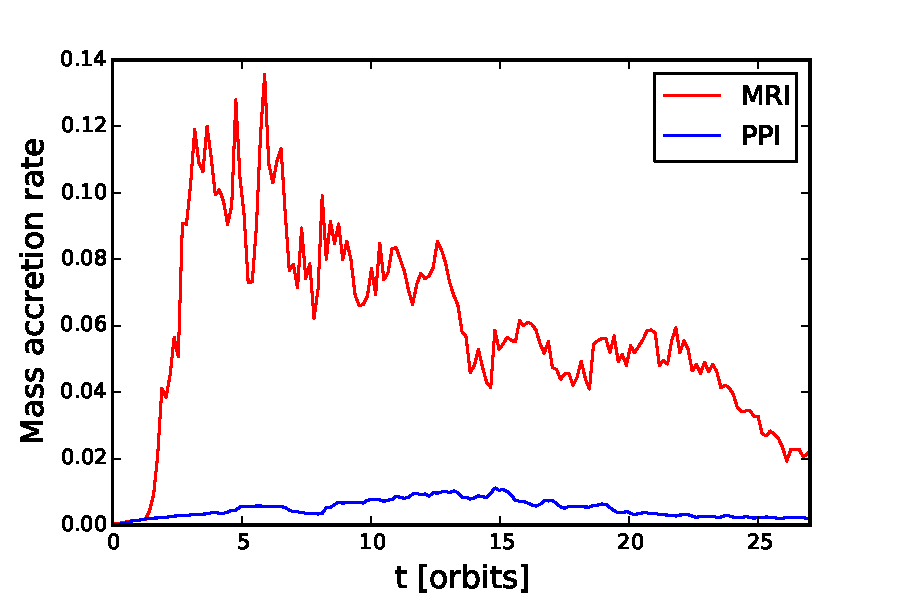
\includegraphics[width=0.45\textwidth,bb=0 0 30 30]{plots/mass_accretion.pdf}
%\caption{The mass accretion rate onto the inner boundary that results from the instabilities.}
%\label{mass_accretion}
%\end{figure}
\section{Introduction}\label{sec:intro}
\par %Introduction: This should describe the physics and give an overview of what you are going to do. Aim to answer the questions: Why would someone want to do this experiment? What is gained?
Brownian motion describes the small random motion of small particles due to their kinetic motion, ---- 
Einstein's ---- work was significant because it served as the one of the first relatively-macroscopic experiment that  proved the atomic nature of matter.The theory of statistical random walk is also important because ---- purely a statistical result--- 
motion from matter composed of atmons  to collide with each other
Jean Perrin's experiment 
particle tracking script  
Then we observe an onion cell under the microscope to observe intracellular transport. We use the ----- compare with the random walk Brownian motion.



\section{Theory}\label{sec:theory}
%Theory: Include the working equations that you will be using but do not include lengthy derivations (such as the Compton or Rutherford formulas) unless specifically asked.where the equations come from and what they are dependent on, (assumptions, conservation laws, etc.), cite reference 
\subsection{Basics}
\par In Einstein's original derivation, he combined the equations that describes osmotic pressure with a series of equations that describes how particles moves through viscous fluids to calculate the theoretical value of D, where D is a dimensionless number called the diffusion coefficient, which describes the extent to which a particle is freely diffusing through the medium without any obstruction. \citep{einstein_1905}\footnote{A more simplified derivation can be found in  \cite{newburgh}.}  
\begin{equation}
D = \frac{k_bT}{3\eta r}
\label{theory}
\end{equation}
where $k_b$ is the Boltzman's constant, T is temperature, $\eta$ is the viscosity of the solution and r is the radius of the particle. Despite the complex derivations, this formula  makes intuitive sense in terms of the familiar kinetic molecular theory(KMT): as the temperature is higher or if the particle size is small, the velocity of the particles are higher, thus the particles collides more rigorously and frequently and more diffusion occurs;  as the solutions gets more viscous, the solution effectively slows the particles down so less diffusion occurs.

\par Since Brownian motion is a series of random walks, it can be modelled as a normal distribution, which means that we can look at the denominator of its exponent to get the variance of the distribution.\citep{math} This mean squared displacement for a list of particle positions, either obtained through simulation or experiment, can also enable us to compute the value of D.
\begin{equation}
D = \sqrt{\langle |\vec{r}(t+\tau)-\vec{r}(t) |\rangle ^2 /2d\tau}
\label{exp}
\end{equation}
where d is the number of dimensions, $\tau$ is the sampling time (0.1 s)
\subsection{Particle Tracking Code}
<briefly explain what code is doing> 
centroid finding 
\subsection{Simulation}
For the particle simulation,  (using code provided in the worksheet) we first create a vector of random steps. We then compute the theoretical D using \ref{theory} to obtain an amplitude (k=$\sqrt{2dD\tau}$, where d = dimensions) for scaling up the random steps. Then using these simulated particle positions, we estimate the value of D using \ref{exp}. Becuase this is a stochastic process, the error depends on $1/\sqrt{N}$, a more detailed error propogation yields the uncertainty quoted in the simulated D values
We used a temperature of 20 degrees Celsius, comparable to our experimental conditions. There is some uncertainty in the temperature because we record only the ambient room temperature and neglect any external heating of the sample due to the microscope light source. However, effects of heating from the microscope should be minimized by our Kohler Illumination setup.
\subsection{Hypothesis}
 We chose to conduct our experiment on  5 different samples, summarized in Table  \ref{table} . Sample \#2 and \#3 enable us to test the effect of viscosity on the Brownian motion, while keeping the particle type and size the same. According to Eq.\ref{sec:theory} and our intuition from KMT, as the viscosity gets larger, there is less random motion and thus Sample \#3 should have a lower value of D.  Sample \#2 and \#4 enable us to compare the particle sizes, and we could similarly infer that Sample \#4 will have a lower value of D. Sample \#2 and \#4 enable us to compare the particle type. While the particle type is not explicitly a variable inside Eq.\ref{sec:theory}, we believe that since glycerol particles are more massive than PVP particle, it will result in slower random walk and therefore a lower value of D. The reasoning behind these experimental choices is that we are only changing one variable per comparison so that we know that the Sample \#2  serve as a standard for comparison. We also chose particle sizes small enough in the range suggested by the lab worksheet so that Brownian motion can actually be observed.
\section{Apparatus and Procedure}\label{sec:ap}
In this experiment we use an inverted compound microscope that is connected to a CCD camera where the image processing is done by a given particle tracking script. Following the procedures:
\begin{enumerate}
\item  We adjust our condenser irises and depth of field to achieve Kohler Illumination to control the amount of light and the incident angle that the light shines on the sample. This setup ensures that the image of the light source is not superposed onto the actual image of the specimen and provides uniform illumination and heating to the sample.  
\item  Then we adjust the condenser so that so that all the illuminating light is blocked off and we only see the light that scatters off the specimen. This technique is called darkfield  illumination and it enables us to look at small particles ($\leq1\mu m$ with the 40x objective) that would otherwise be hard to see with direct illumination.
\item To calibrate the microscope, we make a solution of 10$\mu$m microbeads and water to obtain a pixel-to-meters ratio used in the image-processing script. Since the pixel counting is an error-prone task, we counted the pixel of 3 particles and had both lab members count it, which yields a total of six values, then we averaged these to get an pixel to ratio conversion of 0.48 $\mu m/$pixel for the 20x objective and 0.28$\mu m/$pixel for the 40x objective. (This makes intuitive sense because twice the magnification approximately yields half the pixel ratio.)
\item
%	\begin{itemize}
%	\item 
%	\item 
%	\end{itemize}
\item 
\end{enumerate}
\begin{table*}[t]
\centering
\caption{Experimental condition and results of all trials.}
\label{my-label}
\begin{tabular}{llllll} \label{table}
Trial & Solution Type & Solution viscocity [cp] & Microbead diameter [$\mu m$] & Simulation D          & Experimental D \\
1     & $H_2O$         &  1.00                           & 0.47                              & $1.8184\times 10^{-12}\pm 7.7701\times 10^{-15}$ & $1.9464\times 10^{-12}$     \\
2     & PVP           & 2.50                        & 0.47                              & $7.2988\times 10^{-13}\pm3.2730\times 10^{-15}$ & $1.1515\times 10^{-12}$     \\
3     & PVP           & 4.65                        & 0.47                              & $3.9260\times 10^{-13}\pm1.6801\times 10^{-15}$ & $4.0377\times 10^{-13}$     \\
4     & PVP           & 2.50                        & 1.01                              & $3.3975\times 10^{-13}\pm1.4979\times 10^{-15}$ & $4.3144\times 10^{-13}$     \\
5     & glycerol      & 2.50                        & 0.47                              & $7.3291\times 10^{-13}\pm3.2063\times 10^{-15}$ & $5.0073\times 10^{-13}$    
\end{tabular}
\end{table*}
%Apparatus and Procedure: You should have enough detail so that one familiar with physics but not with the particular experiment at hand could reproduce your experiment if necessary. A block diagram of the equipment is essential here—this should be your own, and not copied out of a book or lab manual. Explain the major pieces of equipment and what they do, but do not overwhelm your reader with details here!
\section{Analysis}\label{sec:analysis}
%Analysis:  the calculations that the lab manual asks you to do are supposed to act as a guide to your analysis, and not as a series of separate calculations. agree with prediction? error analysis? source of error, uncertainty?  
For my analysis, I loaded in the experimental data using the given script \texttt{BrownianMotionParse} and used the Matlab function \texttt{BrownianMotionParse } to write out the parsed data into a textfile. All subsequent dataprocessing is conducted with Python. 
\par A Newtonian fluid is a fluid that has a simple fluid flow behavior where the shear stress is linearly proportional to the viscosity and the shear rate, which means that its viscosity only depends on temperature. The derivation of the diffusion coefficient assumes that the  D is defined assumes that the particle is freely diffusing in aa Newtonian fluid  \cite{Philipse}, so this is why the solutions (water, gyleral and PVP)  we used in this experiemnt are all Newtonian, which gives us the relationship between viscosity, particle size, and diffusion coefficient as described in Sec. \ref{sec:theory}. 
\par From the Newtonian fluid assumption, we can Newton's second law and model the force as a frictional force, which depends linearly on the viscosity. This gives us the Langevin equation (Eq. \ref{lang}) , where the first term comes from the Newtonian derivation (ignoring the term for the random density perturbation in the fluid).
\begin{equation}
\frac{d^2x{dt^2} = \frac{\gamma}{m}\frac{dx}{dt}
\end{equation}where $\gamma  = 6\pi \eta a$.
Solving this differential equation yields the solution of form :
\begin{equation}
v(t) = e^{-t/\tau_B} v(0)
\end{equation}
We ignore the exponential component of the general solution because if we do a detailed calculation, we will find that Brownian motion is essentially a Markov (i.e. random) process, because there are as much as $10^{11}$ collisions during the 0.1 seconds time period that we are sampling that the effects of any interparticle correlation or interaction due to an external potential will not sustain. 
I computed the autocorrelation by computing the correlation between two adjacent positions:
\begin{equation}
corr(k) = \Sum^N_{i=1} x_{i} * x_{i+k}
\end{equation} and obtained an average correlation of -0.00792\pm 0.12525 to confirm that the diffusion process is largely random. The small nonzero autocorrelation may result from bulk flow due to uneven heating or elevation of the microscope slides. 
\par Knowing that these particle motion are largely due to Brownian motion, we want to verify whether Eq. \ref{exp} holds true. We by summing up 

\par If the particle is in a mesh or network, like in our onion cell intracellular example, we don't expect to see Brownian diffusion, because the motion is constrained along the tubules so the particle motion is not a random process.
\subsection{Molecular Motors}
\section{Conclusion}\label{sec:conclusion}
%findings, future improvement? 
 
\acknowledgments
\section*{Acknowledgments}
I am sincerely thankful for support from Professor Harmut Haeffner, Kam-Biu Luk, Don Orlando, and my lab partner Xiyue Wang for contributing to successful completion of this lab.
\bibliography{bibdatabase}
%Raw Data: You must include the data that you took in lab in an appendix; the data should be clear enough so that someone could look at it and determine what you measured and how you measured it. You should be keeping a lab notebook, so simply photocopy all relevant pages. Your report should include all of the listed sections, along with the signed Pre-lab and Mid–Lab Discussion sheets.
\end{document}


